\documentclass[aspectratio=169,11pt]{beamer}
% Theme
\usetheme{Berlin}
\usecolortheme{dolphin}
\setbeamertemplate{navigation symbols}{}
\setbeamertemplate{footline}[frame number]
\usepackage[utf8]{inputenc}
\usepackage[T1]{fontenc}
% \usepackage[french]{babel} % activez si texlive-lang-french est installé
\usepackage{lmodern}
\usepackage{amsmath}
\usepackage{booktabs}
\usepackage{tabularx}
\usepackage{array}
\usepackage{graphicx}
\usepackage{xcolor}
\usepackage{ragged2e}
\usepackage{pgfplots}
\usepackage{tikz}
\usetikzlibrary{arrows.meta,positioning,shapes.geometric}
\pgfplotsset{compat=1.18}
% Colors
\definecolor{myblue}{RGB}{35,55,120}
\definecolor{myred}{RGB}{150,60,60}
\definecolor{mygreen}{RGB}{45,110,85}
\definecolor{mygray}{RGB}{90,90,90}
\setbeamercolor{title}{fg=myblue}
\setbeamercolor{frametitle}{fg=white,bg=myblue}
\setbeamercolor{structure}{fg=myblue}
\setbeamercolor{section in head/foot}{bg=myblue,fg=white}
\setbeamercolor{subsection in head/foot}{bg=myblue!80,fg=white}
\setbeamercolor{title in head/foot}{bg=myblue,fg=white}
\setbeamercolor{author in head/foot}{bg=myblue!85,fg=white}
\setbeamercolor{date in head/foot}{bg=myblue!85,fg=white}
\setbeamercolor{block title}{bg=myblue,fg=white}
\setbeamercolor{block body}{bg=blue!5,fg=black}
\setbeamercolor{itemize item}{fg=myblue}
\setbeamercolor{itemize subitem}{fg=myblue}

\title[Banque de données spatio-temporelles]{Constitution d'une banque de données de référence pour la validation de modèles prédictifs spatio-temporels}
\author{Johnny D'OLIVEIRA}
\institute{Aix-Marseille School of Economics \\ \small Stage INRAE Avignon --- Unité Écodéveloppement \\ \small Encadrant : Ghislain Geniaux}
\date{9 juin 2026}

\begin{document}

\begin{frame}
    \titlepage
\end{frame}

\begin{frame}{Plan}
    \tableofcontents
\end{frame}

% ============================================================
\section{Contexte et problème}
% ============================================================
\begin{frame}{Contexte : des méthodes qui ont besoin d'être validées}
\small
L'INRAE d'Avignon développe des méthodes statistiques avancées pour les données
\textbf{spatiales} et \textbf{spatio-temporelles}
(packages R maison : \texttt{mgwrsar}, \texttt{spboost}).
\vspace{0.2cm}

Pour démontrer qu'une méthode est robuste et prédictive, les publications
s'appuient sur \textbf{trois étapes complémentaires} :
\begin{itemize}
    \item étudier ses \textbf{propriétés asymptotiques} mathématiquement \hfill{\footnotesize\textcolor{mygray}{(quand cela est possible)}}
    \item la tester sur des \textbf{données simulées} avec de nombreuses répétitions :
    on connaît alors le vrai mécanisme et les vrais effets
    \hfill{\footnotesize\textcolor{mygray}{(Monte-Carlo)}}
    \item la confronter à des \textbf{données réelles et variées} :
    on observe sa capacité à fonctionner dans des situations concrètes
    \hfill{\footnotesize\textcolor{mygray}{(souvent 1 à 2 cas)}}
\end{itemize}
\vspace{0.2cm}
\begin{block}{Le problème}
Il n'existe pas de jeux de données \textbf{standardisés et diversifiés en grand nombre}, en spatial et en spatio-temporel.
\end{block}
\end{frame}

\begin{frame}{Un jeu de données idéal : des données reliées à leurs usages}
\scriptsize
\centering
\begin{tikzpicture}[
    source/.style={draw=myblue!55, rounded corners=2pt, fill=blue!3,
        minimum width=2.75cm, text width=2.5cm, align=center, inner sep=3pt},
    data/.style={draw=mygreen!80, rounded corners=2pt, very thick, fill=mygreen!5,
        minimum width=7.0cm, text width=6.7cm, align=center, inner sep=4pt},
    link/.style={-{Latex[length=2mm]}, thick, myblue},
    linklabel/.style={fill=white, inner sep=1pt, text=mygray, font=\tiny}
]
% Figurine de l'article scientifique
\node[source] (article) at (0,0.4) {
    \includegraphics[page=1,width=1.55cm,height=1.95cm,keepaspectratio]
        {assets/muenchow2012_lsl.pdf}\\[-1mm]
    \textbf{Article scientifique}\\
    Muenchow, Brenning \& Richter (2012)\\
    {\tiny \emph{Geomorphology}}
};

% Dataset central : valeurs réelles de head(lsl)
\node[data] (dataset) at (5.25,0.45) {
    \textbf{\large \texttt{spDataLarge::lsl}}\\[-1mm]
    {\tiny 350 observations --- glissements de terrain, sud de l'Équateur}\\[1mm]
    \resizebox{6.45cm}{!}{%
    \begin{tabular}{rrrrrr}
    \toprule
    \textbf{lslpts} & \textbf{slope} & \textbf{cplan} &
    \textbf{cprof} & \textbf{elev} & \textbf{log10\_carea}\\
    \midrule
    FALSE & 33.75 &  0.0232 &  0.0032 & 2422.8 & 2.784\\
    FALSE & 39.41 & -0.0386 & -0.0172 & 2051.8 & 4.146\\
    FALSE & 37.45 & -0.0133 &  0.0097 & 1957.8 & 3.644\\
    FALSE & 31.50 &  0.0409 &  0.0059 & 1968.6 & 2.269\\
    FALSE & 44.07 &  0.0097 &  0.0051 & 3007.8 & 3.003\\
    \bottomrule
    \end{tabular}}\\[-0.5mm]
    {\tiny Extrait réel obtenu avec \texttt{head(lsl)}}
};

% Figurine du livre / chapitre
\node[source] (book) at (10.55,1.35) {
    \includegraphics[page=1,width=1.45cm,height=1.55cm,keepaspectratio]
        {assets/geocomputation_with_r.pdf}\\[-1mm]
    \textbf{Geocomputation with R}\\
    {\tiny chapitre \emph{Statistical learning for geographic data}}\\[-0.5mm]
    {\tiny\color{myred}\textbf{Forme R directement exploitable}}
};

% Figurine du package R
\node[source] (package) at (10.55,-1.45) {
    {\color{myblue}\fontsize{24}{24}\selectfont\textbf{R}}\\[-1mm]
    \textbf{Package \texttt{spDataLarge}}\\
    {\tiny fournit et documente le dataset \texttt{lsl}}
};

% Relations explicites
\draw[link] (article.east) -- node[linklabel,above]{utilise / documente} (dataset.west);
\draw[link] (package.west) -- (dataset.south east);
\draw[link] (book.west) -- node[linklabel,above]{utilise} (dataset.north east);

% Formule issue du chapitre en ligne
\node[draw=myred!70, rounded corners=2pt, fill=myred!5,
      text width=7.0cm, align=center, inner sep=3pt]
      (formula) at (5.25,-2.35) {
    \textbf{Formule de modélisation et localisation :}\\[-1mm]
    $\texttt{lslpts} \sim \texttt{slope}+\texttt{cplan}+\texttt{cprof}
       +\texttt{elev}+\texttt{log10\_carea}$\\[-0.5mm]
    {\tiny chaque observation $i$ est localisée par
    $\mathbf{s}_i=(\texttt{x}_i,\texttt{y}_i)$}
};
\draw[link,myred] (article.south east)
    .. controls (1.4,-0.8) and (2.1,-2.15) ..
    node[linklabel,below left]{modèle publié}
    (formula.west);
\draw[link,dashed,mygray] (book.south west)
    .. controls (8.85,0.15) and (9.15,-2.15) ..
    node[linklabel,right]{forme R directement exploitable}
    (formula.east);
\end{tikzpicture}
\end{frame}

\begin{frame}{Objectif du stage}
\small
\begin{block}{Question directrice}
Comment construire une banque de données spatio-temporelles \emph{diversifiée, documentée et réutilisable} pour comparer équitablement des modèles prédictifs --- \textbf{en utilisant l'IA pour automatiser sa conception et faciliter sa mise à jour} ?
\end{block}
\vspace{0.2cm}
\textbf{Trois axes de travail}
\begin{enumerate}
    \item \textbf{Collecte \& curation} : récolter des jeux ouverts (entrepôts scientifiques, open data) couvrant des domaines variés.
    \item \textbf{Structuration} : architecture de stockage standardisée + protocoles de séparation Train/Test/Validation.
    \item \textbf{Modélisation \& benchmarking} : baselines classiques (GLM, GAM), modèles spatiaux (SAR, MGWR) et Machine Learning.
\end{enumerate}
\end{frame}

\begin{frame}{Où chercher les données ? Trois étages}
\small
La collecte s'organise en trois familles de sources complémentaires.
\vspace{0.3cm}
\begin{enumerate}
    \item \textbf{Packages R / Python} \\
    {\footnotesize Jeux spatiaux et spatio-temporels embarqués dans les librairies (\texttt{spData}, \texttt{sf}, \texttt{mgwrsar}\dots). \emph{Étage prioritaire} : le mieux documenté et le plus contrôlé.}
    \vspace{0.2cm}
    \item \textbf{Articles scientifiques} \\
    {\footnotesize Jeux publiés en open source par des articles de statistique / économétrie spatiale et spatio-temporelle.}
    \vspace{0.2cm}
    \item \textbf{Banques de données et portails} \\
    {\footnotesize Jeux spatiaux et spatio-temporels des entrepôts institutionnels (INSEE, Eurostat, Zenodo, Dryad\dots).}
\end{enumerate}
\end{frame}

% ============================================================
\section{Idée directrice : des métadonnées qui guident}
% ============================================================
\begin{frame}{L'idée centrale : décrire ne suffit pas}
\small
\begin{itemize}
    \item Habituellement, on \emph{décrit} un jeu de données (titre, source, taille).
    \vspace{0.2cm}
    \item Notre idée : construire des \textbf{métadonnées enrichies} qui \emph{guident automatiquement} les choix méthodologiques.
\end{itemize}
\vspace{0.4cm}
\begin{center}
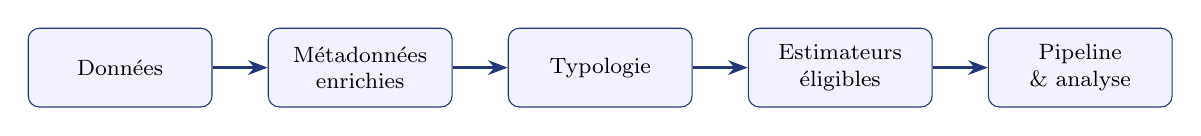
\begin{tikzpicture}[
    node distance=0.55cm and 0.7cm,
    box/.style={rectangle, rounded corners, draw=myblue, fill=blue!5,
                text width=2.1cm, align=center, minimum height=1cm, font=\footnotesize},
    arr/.style={-{Stealth[length=2.5mm]}, myblue, thick}]
\node[box] (a) {Données};
\node[box, right=of a] (b) {Métadonnées enrichies};
\node[box, right=of b] (c) {Typologie};
\node[box, right=of c] (d) {Estimateurs éligibles};
\node[box, right=of d] (e) {Pipeline \& analyse};
\draw[arr] (a)--(b);
\draw[arr] (b)--(c);
\draw[arr] (c)--(d);
\draw[arr] (d)--(e);
\end{tikzpicture}
\end{center}
\vspace{0.2cm}
\footnotesize \centering Le fil conducteur méthodologique : \textbf{donnée $\rightarrow$ métadonnée $\rightarrow$ typologie $\rightarrow$ modèle $\rightarrow$ analyse}.
\end{frame}

\begin{frame}{Les six blocs de métadonnées enrichies}
\footnotesize
\begin{tabularx}{\textwidth}{>{\RaggedRight\arraybackslash}p{0.30\textwidth} >{\RaggedRight\arraybackslash}X}
\toprule
\textbf{Bloc} & \textbf{Ce qu'il capture} \\
\midrule
1. Formule \& variables & Variable réponse Y, explicatives X, formule (publiée vs reconstruite) \\
2. Identification \& DOI & Traçabilité : DOI dataset, DOI publication, source, script \\
3. Typologie des modèles & Tâche (régression / classification), famille, variante \\
4. Typologie des données & Spatial / spatio-temporel, panel, type de Y, profil N/T \\
5. Résolution \& étendue & Grain (commune, parcelle, grille) et emprise spatiale/temporelle \\
6. Reproductibilité & Code disponible, dépôt, licence \\
\bottomrule
\end{tabularx}
\vspace{0.25cm}
\begin{itemize}
    \item Inspiration : le package R \texttt{caret} (registre de modèles), mais en \emph{reliant} données et estimateurs.
\end{itemize}
\end{frame}

\begin{frame}{Une typologie des jeux de données en 6 axes}
\footnotesize
La banque n'est pas une accumulation : c'est un \textbf{plan d'expérience}. Chaque jeu est positionné selon 6 axes orthogonaux.
\vspace{0.25cm}
\begin{columns}
\column{0.5\textwidth}
\begin{enumerate}
    \item \textbf{Domaine} (immobilier, climat, santé\dots)
    \item \textbf{Support spatial} (points, polygones, grille, réseau)
    \item \textbf{Structure temporelle} (coupe, panel, séries)
\end{enumerate}
\column{0.5\textwidth}
\begin{enumerate}
    \setcounter{enumi}{3}
    \item \textbf{Type de réponse Y} (continue, comptage, binaire\dots)
    \item \textbf{Dépendance} (autocorrélation, hétérogénéité, diffusion)
    \item \textbf{Taille} (N, T, nombre de covariables)
\end{enumerate}
\end{columns}
\vspace{0.3cm}
\centering\small Objectif : couvrir au moins 5 domaines et 5 types de réponse distincts.
\end{frame}

% ============================================================
\section{Le système et son ingénierie}
% ============================================================
\begin{frame}{Le défi : collecter à grande échelle}
\begin{itemize}
    \item Des centaines de jeux candidats, dispersés dans des entrepôts et des articles.
    \vspace{0.2cm}
    \item Remplir manuellement les métadonnées de chacun serait \textbf{trop long}.
    \vspace{0.2cm}
    \item Un assistant IA peut automatiser les tâches répétitives :
    \textbf{lire, extraire, résumer, ranger et relier}.
    \vspace{0.2cm}
    \item Mais s'il relit tout le corpus à chaque tâche, le coût explose :
    un \textbf{token} est l'unité de texte traitée et facturée par l'IA.
\end{itemize}
\vspace{0.3cm}
\centering\emph{Il faut un bibliothécaire qui mémorise son classement,
pas un bibliothécaire qui relit tous les rayons à chaque question.}
\end{frame}

\begin{frame}{Le système en pratique}
\footnotesize
\begin{block}{Une mémoire cumulative pour l'assistant IA}
Au lieu de relire toutes les sources à chaque question, l'IA construit une base
structurée et des synthèses validables, puis les maintient à jour.
\end{block}
\vspace{0.05cm}
\begin{columns}
\column{0.39\textwidth}
\textbf{Trois couches complémentaires}
\begin{itemize}
    \item \textbf{Corpus} : les articles, documentations et données d'origine.
    \item \textbf{Graphe de connaissances} : des \emph{nœuds}
    (article, dataset, formule) reliés par des relations
    (\emph{utilise}, \emph{fournit}, \emph{explique}).
    \item \textbf{Wiki} : des fiches en langage naturel, relisibles et validables par l'humain.
\end{itemize}
\column{0.61\textwidth}
\centering
\resizebox{0.95\linewidth}{!}{%
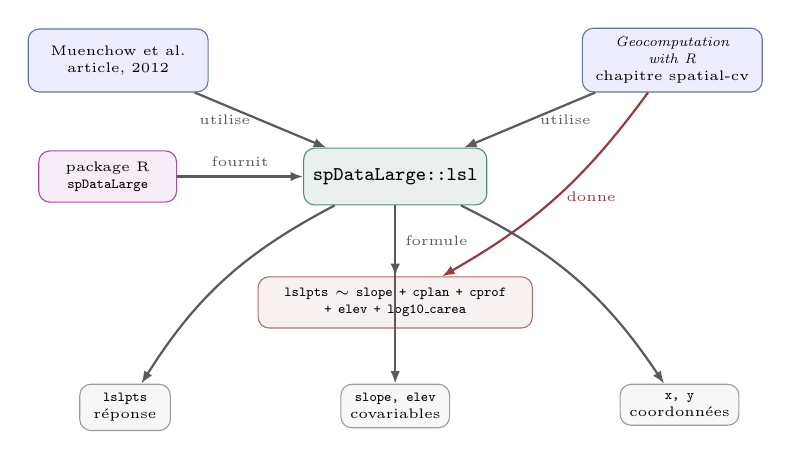
\begin{tikzpicture}[
    node distance=6mm and 8mm,
    every node/.style={font=\tiny, align=center},
    dataset/.style={draw=mygreen!80, fill=mygreen!10, rounded corners,
        minimum width=2.0cm, minimum height=0.72cm, font=\scriptsize\bfseries},
    paper/.style={draw=myblue!70, fill=blue!7, rounded corners,
        text width=2.05cm, minimum height=0.8cm},
    package/.style={draw=violet!70, fill=violet!7, rounded corners,
        minimum width=1.75cm, minimum height=0.65cm},
    formula/.style={draw=myred!75, fill=myred!7, rounded corners,
        text width=3.25cm, minimum height=0.65cm},
    varnode/.style={draw=mygray!60, fill=black!3, rounded corners,
        minimum width=1.15cm, minimum height=0.52cm},
    edge/.style={-{Latex[length=1.6mm]}, thick, mygray}
]
\node[dataset] (lsl) {\texttt{spDataLarge::lsl}};
\node[paper, above left=7mm and 12mm of lsl] (article)
    {Muenchow et al.\\article, 2012};
\node[paper, above right=7mm and 12mm of lsl] (book)
    {\emph{Geocomputation with R}\\chapitre spatial-cv};
\node[package, left=16mm of lsl] (pkg) {package R\\\texttt{spDataLarge}};
\node[formula, below=9mm of lsl] (form)
    {\texttt{lslpts} $\sim$ \texttt{slope + cplan + cprof}\\
     \texttt{+ elev + log10\_carea}};
\node[varnode, below left=7mm and 11mm of form] (y)
    {\texttt{lslpts}\\réponse};
\node[varnode, below=7mm of form] (x)
    {\texttt{slope, elev}\\covariables};
\node[varnode, below right=7mm and 11mm of form] (xy)
    {\texttt{x, y}\\coordonnées};

\draw[edge] (pkg) -- node[above]{fournit} (lsl);
\draw[edge] (article) -- node[left]{utilise} (lsl);
\draw[edge] (book) -- node[right]{utilise} (lsl);
\draw[edge,myred] (book) to[bend left=12] node[right]{donne} (form);
\draw[edge] (lsl) -- node[right]{formule} (form);
\draw[edge] (lsl) to[bend right=15] (y);
\draw[edge] (lsl) -- (x);
\draw[edge] (lsl) to[bend left=15] (xy);
\end{tikzpicture}
}

{\tiny\textcolor{mygray}{Le graphe oriente d'abord l'IA vers les bonnes sources ;
le wiki lui fournit ensuite une synthèse contrôlable.}}
\end{columns}
\end{frame}

\begin{frame}{Garder la qualité : un contrôle à trois niveaux}
\small
Chaque fiche produite par l'IA passe un contrôle qualité automatique avant d'être validée.
\vspace{0.3cm}
\begin{tabularx}{\textwidth}{>{\RaggedRight\arraybackslash}p{0.22\textwidth} >{\RaggedRight\arraybackslash}X c}
\toprule
\textbf{Niveau} & \textbf{Vérifie} & \textbf{Feu} \\
\midrule
Structurel & Forme : sections obligatoires, liens valides & \textcolor{mygreen}{$\bullet$} \\
Sémantique & Cohérence du contenu, fidélité à la source & \textcolor{myred}{$\bullet$} \\
File d'attente & Cas douteux orientés vers \textbf{révision humaine} & \textcolor{orange}{$\bullet$} \\
\bottomrule
\end{tabularx}
\vspace{0.3cm}
\begin{itemize}
    \item Principe clé : \textbf{l'IA propose, l'humain valide}. Aucune auto-validation.
\end{itemize}
\end{frame}

\begin{frame}{La solution : donner une mémoire et des résumés à l'IA}
\footnotesize
\begin{columns}
\column{0.43\textwidth}
On a ajouté des outils qui évitent à l'IA de tout relire :
\begin{itemize}
    \item un \textbf{graphe de connaissances} qu'on interroge au lieu de relire les sources ;
    \item des \textbf{résumés} des sources et des longues sorties techniques ;
    \item une \textbf{compression} du contexte avant chaque appel.
\end{itemize}
\vspace{0.1cm}
\textbf{Exemple de volume évité :}\\
pour retrouver les sources reliées à \texttt{lsl}

\column{0.57\textwidth}
\centering
\begin{tikzpicture}
\begin{axis}[
    width=\textwidth, height=0.48\textheight,
    ybar, bar width=25pt,
    symbolic x coords={Fichiers sources,Requête KG},
    xtick=data,
    ymode=log,
    ymin=100, ymax=1000000,
    ylabel={Volume estimé (tokens, échelle log.)},
    nodes near coords,
    point meta=explicit symbolic,
    nodes near coords style={font=\scriptsize},
    tick label style={font=\scriptsize},
    label style={font=\scriptsize},
    x tick label style={align=center}]
\addplot[fill=myred!75] coordinates
    {(Fichiers sources,521443) [\scriptsize $\approx$521\,000]
     (Requête KG,722) [\scriptsize $\approx$720]};
\end{axis}
\end{tikzpicture}
\\[-0.05cm]
\colorbox{mygreen!12}{\parbox{0.88\linewidth}{\centering
\textbf{Requête locale dans le KG :} environ \textbf{0,12 seconde}}}
\end{columns}
\vspace{0.05cm}

{\tiny\textcolor{mygray}{Le graphique compare le volume de texte accessible,
pas la qualité finale des réponses. Estimation : caractères divisés par 4 ;
ce n'est pas un relevé de facturation API.}}
\end{frame}

% ============================================================
\section{Application et premiers résultats}
% ============================================================
\begin{frame}{État d'avancement de la banque}
\footnotesize
\centering
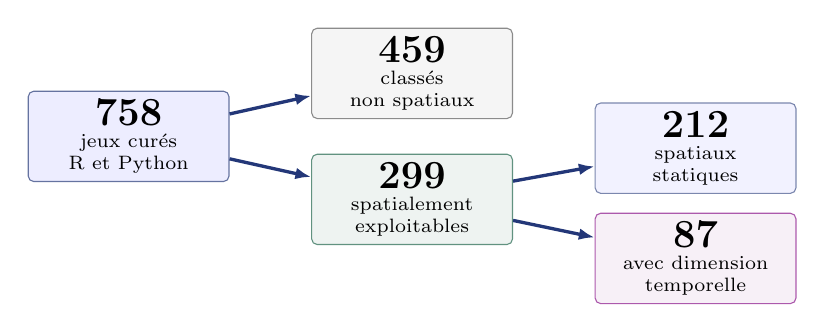
\begin{tikzpicture}[
    metric/.style={rounded corners=2pt, minimum width=2.55cm,
        minimum height=1.05cm, text width=2.3cm, align=center,
        font=\scriptsize, inner sep=3pt},
    flow/.style={-{Latex[length=2mm]}, very thick, myblue}
]
\node[metric, draw=myblue!70, fill=blue!7] (all) at (0,0)
    {\textbf{\Large 758}\\jeux curés\\R et Python};
\node[metric, draw=mygray!70, fill=black!4] (nonsp) at (3.6,0.8)
    {\textbf{\Large 459}\\classés\\non spatiaux};
\node[metric, draw=mygreen!75, fill=mygreen!8] (sp) at (3.6,-0.8)
    {\textbf{\Large 299}\\spatialement\\exploitables};
\node[metric, draw=myblue!60, fill=blue!5] (static) at (7.2,-0.15)
    {\textbf{\Large 212}\\spatiaux\\statiques};
\node[metric, draw=violet!65, fill=violet!6] (st) at (7.2,-1.55)
    {\textbf{\Large 87}\\avec dimension\\temporelle};
\draw[flow] (all) -- (nonsp);
\draw[flow] (all) -- (sp);
\draw[flow] (sp) -- (static);
\draw[flow] (sp) -- (st);
\end{tikzpicture}

\vspace{0.08cm}
\begin{columns}[T]
\column{0.49\textwidth}
\centering
\textbf{Taille $N$ des 299 jeux spatiaux}\\[1mm]
\begin{tabular}{lr}
\toprule
Observations & Jeux \\
\midrule
$N<100$ & 110\\
$100\leq N<1\,000$ & 109\\
$N\geq1\,000$ & 80\\
\bottomrule
\end{tabular}
\column{0.49\textwidth}
\centering
\textbf{Nombre de variables $K$}\\[1mm]
\begin{tabular}{lr}
\toprule
Variables & Jeux \\
\midrule
$K\leq10$ & 142\\
$11\leq K\leq50$ & 109\\
$K>50$ & 48\\
\bottomrule
\end{tabular}
\end{columns}
\vspace{0.08cm}

{\scriptsize\textcolor{myred}{Seulement 21 jeux ont $K>N$ :
la haute dimension reste encore peu couverte.}}
\end{frame}

\begin{frame}{Les modèles à comparer}
\small
Un portefeuille gradué, du plus simple au plus spécialisé.
\vspace{0.3cm}
\begin{tabularx}{\textwidth}{>{\RaggedRight\arraybackslash}p{0.26\textwidth} >{\RaggedRight\arraybackslash}X}
\toprule
\textbf{Niveau} & \textbf{Modèles} \\
\midrule
1. Baselines & GLM, GAM, Random Forest, Gradient Boosting \\
2. Spatiaux statiques & SAR / SEM, GWR / MGWR, \texttt{spboost} \\
3. Spatio-temporels & Panel spatial, GTWR / MGTWR, MGTWRSAR, STVC \\
\bottomrule
\end{tabularx}
\vspace{0.3cm}
\begin{itemize}
    \item \textbf{RMSE / MAE} : taille moyenne des erreurs de prédiction.
    \item \textbf{Moran des résidus} : vérifie s'il reste une autocorrélation spatiale non expliquée.
    \item \textbf{Temps de calcul} : critère important pour les grands jeux de données.
    \item Les méthodes maison (\texttt{spboost}, MGTWRSAR) sont comparées aux références.
\end{itemize}
\end{frame}

% ============================================================
\section{Calendrier et conclusion}
% ============================================================
\begin{frame}{Où en est-on, et la suite}
\small
\begin{itemize}
    \item \textbf{Fait} : typologie, pipelines de collecte, contrôle qualité, couche d'efficience (tokens).
    \vspace{0.15cm}
    \item \textbf{En cours} : curation, dédoublonnage et mesure de la couverture réelle de la banque.
    \vspace{0.15cm}
    \item \textbf{À venir} : combler les catégories sous-représentées,
    définir les protocoles Train/Test, puis lancer le benchmarking.
    \vspace{0.15cm}
    \item \textbf{Finalité} : un \emph{datapaper} (cible : \textit{Scientific Data}) + dépôt Zenodo + code GitHub.
\end{itemize}
\end{frame}

\begin{frame}{Conclusion}
\small
Ce stage construit une banque de données spatio-temporelles de référence pour valider des méthodes prédictives.
\vspace{0.3cm}
\textbf{Trois messages à retenir}
\begin{itemize}
    \item Des \textbf{métadonnées enrichies} qui ne décrivent pas seulement, mais \emph{guident} le choix des modèles.
    \vspace{0.15cm}
    \item Un \textbf{graphe de connaissances et un wiki} pour orienter l'IA,
    stabiliser les résultats et permettre leur validation humaine.
    \vspace{0.15cm}
    \item Une \textbf{ingénierie d'efficience} (économie de tokens) qui a débloqué le projet.
\end{itemize}
\end{frame}

\section*{}
\begin{frame}[plain]
  \begin{center}
    {\Huge Thank you}\\[1em]
    {\large Johnny D'OLIVEIRA}\\[0.3em]
    Aix-Marseille School of Economics\\[0.3em]
    INRAE-Ecodeveloppement
  \end{center}
\end{frame}

\end{document}
